\def\documentauthor{Carlos Salinas}
\def\documenttitle{MA 166: Quiz \hwnum}
\def\hwnum{3}
\def\shorttitle{MA 166 HW \hwnum}
\def\coursename{MA166}
\def\documentsubject{calculus ii}
\def\authoremail{salinac@purdue.edu}

\documentclass[12pt]{article}
\usepackage{geometry}
\usepackage[dvipsnames]{xcolor}
\usepackage[
    breaklinks,
    bookmarks=true,
    colorlinks=true,
    pageanchor=false,
    linkcolor=black,
    anchorcolor=black,
    citecolor=black,
    filecolor=black,
    menucolor=black,
    runcolor=black,
    urlcolor=black,
    hyperindex=false,
    hyperfootnotes=true,
    pdftitle={\shorttitle},
    pdfauthor={\documentauthor},
    pdfkeywords={\documentsubject},
    pdfsubject={\coursename}
    ]{hyperref}

% Use symbols instead of numbers
\renewcommand*{\thefootnote}{\fnsymbol{footnote}}

%% Math
\usepackage{amsmath}
\usepackage{amsthm}
\usepackage{amssymb}
\usepackage{mathtools}

%%PDFTeX specific
\usepackage[mathcal]{euscript}
\usepackage{mathrsfs}
\usepackage{dsfont}
\usepackage{wasysym}

\usepackage[LAE,LFE,T2A,T1]{fontenc}
\usepackage[utf8]{inputenc}
\usepackage[farsi,french,german,spanish,russian,english]{babel}
\babeltags{pa=farsi,
           fr=french,
           de=german,
           es=spanish,
           ru=russian,
           en=english}
\def\spanishoptions{mexico}

\selectlanguage{english}

\newcommand{\textfa}[1]{\beginR\textpa{#1}\endR}

\usepackage{cmap}
\usepackage{CJKutf8}
\newcommand{\textkr}[1]{\begin{CJK}{UTF8}{mj}#1\end{CJK}}
\newcommand{\textjp}[1]{\begin{CJK}{UTF8}{min}#1\end{CJK}}
\newcommand{\textzh}[1]{\begin{CJK}{UTF8}{bsmi}#1\end{CJK}}

%% Misc
\usepackage{graphicx}
\usepackage{cutwin}
\graphicspath{{figures/}}

\usepackage{microtype}
\usepackage{multicol}
\usepackage[inline]{enumitem}
\usepackage{listings}
\usepackage{mleftright}
\mleftright

%% Theorems and definitions
\theoremstyle{plain}
\newtheorem{theorem}{Theorem}
\newtheorem{proposition}[theorem]{Proposition}
\newtheorem{corollary}[theorem]{Corollary}
\newtheorem{claim}[theorem]{Claim}
\newtheorem{lemma}[theorem]{Lemma}
\newtheorem{axiom}[theorem]{Axiom}

\newtheorem*{corollary*}{Corollary}
\newtheorem*{claim*}{Claim}
\newtheorem*{lemma*}{Lemma}
\newtheorem*{proposition*}{Proposition}
\newtheorem*{theorem*}{Theorem}

\theoremstyle{definition}
\newtheorem{definition}{Definition}
\newtheorem{example}{Examples}
\newtheorem{examples}[example]{Examples}
\newtheorem{exercise}{Exercise}
\newtheorem{problem}[exercise]{Problem}

\newtheorem*{definition*}{Definition}
\newtheorem*{example*}{Examples}
\newtheorem*{examples*}{Examples}
\newtheorem*{exercise*}{Exercise}
\newtheorem*{problem*}{Problem}

\theoremstyle{remark}
\newtheorem{remark}{Remark}
\newtheorem{remarks}[remark]{Remarks}
\newtheorem{observation}[remark]{Observation}
\newtheorem{observations}[remark]{Observations}

\newtheorem*{remark*}{**Remark**}
\newtheorem*{remarks*}{**Remarks**}
\newtheorem*{observation*}{**Observation**}
\newtheorem*{observations*}{**Observations**}

%% Commands and operators
%% Redefinitions & commands
\newcommand{\nsubset}{\ensuremath{\not\subset}}
\newcommand{\nsupset}{\ensuremath{\not\supset}}
\newcommand\minus{\ensuremath{\null\smallsetminus}}
\renewcommand\qedsymbol{\ensuremath{\null\hfill\blacksquare}}

%% Commands and operators
\DeclareMathOperator{\id}{id}
\DeclareMathOperator{\im}{im}

%% Linear algebra
\DeclareMathOperator{\proj}{proj}
\DeclareMathOperator{\comp}{comp}

%% Differential operators
\DeclareMathOperator{\Curl}{curl}
\DeclareMathOperator{\Div}{div}
\DeclareMathOperator{\Grad}{grad}
\DeclareMathOperator{\Lap}{\Delta}
\DeclareMathOperator{\diff}{d\!}

%% Misc
\newcommand{\bbC}{\mathbb{C}}
\newcommand{\bbCP}{\mathbb{CP}}
\newcommand{\bbH}{\mathbb{H}}
\newcommand{\bbN}{\mathbb{N}}
\newcommand{\bbQ}{\mathbb{Q}}
\newcommand{\bbR}{\mathbb{R}}
\newcommand{\bbRP}{\mathbb{RP}}
\newcommand{\bbZ}{\mathbb{Z}}

\newcommand{\bfC}{\mathbf{C}}
\newcommand{\bfCP}{\mathbf{CP}}
\newcommand{\bfH}{\mathbf{H}}
\newcommand{\bfN}{\mathbf{N}}
\newcommand{\bfQ}{\mathbf{Q}}
\newcommand{\bfR}{\mathbf{R}}
\newcommand{\bfRP}{\mathbf{RP}}
\newcommand{\bfZ}{\mathbf{Z}}

\newcommand{\calA}{\mathcal{A}}
\newcommand{\calB}{\mathcal{B}}
\newcommand{\calC}{\mathcal{C}}
\newcommand{\calS}{\mathcal{S}}
\newcommand{\calT}{\mathcal{T}}
\newcommand{\calU}{\mathcal{U}}
\newcommand{\calV}{\mathcal{V}}

\newcommand{\scrL}{\mathscr{L}}
\newcommand{\scrO}{\mathscr{O}}
\newcommand{\scrS}{\mathscr{S}}

\newcommand{\bfa}{\mathbf{a}}
\newcommand{\bfb}{\mathbf{b}}
\newcommand{\bfc}{\mathbf{c}}
\newcommand{\bfu}{\mathbf{u}}
\newcommand{\bfv}{\mathbf{v}}
\newcommand{\bfw}{\mathbf{w}}

\begin{document}
\author{TA: \href{mailto:\authoremail}{\documentauthor}}
\title{\documenttitle}
\date{\today}
\maketitle

You have \textbf{15 minutes} to complete this quiz. You may work in groups,
but you are not allowed to use any other resources.
\\\\
%% Quiz problems
\begin{problem}
\label{prob:1}
Let $\bfu=\langle 6,3,1\rangle$, $\bfv=\langle 0,1,2\rangle$, and
$\bfw=\langle 4,-2,5\rangle$.
\begin{enumerate}[label=(\roman*)]
\item \label{prob:1-i}Find the scalar projection $\comp_{\bfv}\bfw$.
\item \label{prob:1-ii} Find the projection $\proj_{\bfu}\bfv$.
\item \label{prob:1-iii} Find the cross product $\bfv\times\bfw$.
\item \label{prob:1-iv} What is a vector orthogonal to $\bfv$ and $\bfw$?
\item \label{prob:1-v}Find the scalar triple product $\bfu\cdot(\bfv\times\bfw)$.
\item \label{prob:1-vi} Are the vectors $\bfu$, $\bfv$, and $\bfw$ coplanar?
\end{enumerate}
\end{problem}
\bigskip
\begin{problem}% [MA 166, Exam 1, Fall 2015]
\label{prob:2}
Find the area enclosed by the regions
\begin{enumerate}[label=(\roman*)]
\item \label{prob:2-i} $y=x^3$, and $y=|x|$.
\item \label{prob:2-ii} $y=e^x$, $y=e^2x$, and $x=\ln 2$.
\end{enumerate}
\end{problem}
\newpage
\section*{Solutions}
\begin{proof}[Solution to Problem \ref{prob:1}]
\ref{prob:1-i} Recall the formula for the scalar projection of the vector
$\bfb$ onto $\bfa$
\begin{equation}
\label{eq:scalar-projection}
\comp_{\bfa}\bfb=\frac{\bfa\cdot\bfb}{|\bfa|}.
\end{equation}
All we need to do for this problem is to substitute $\bfv$ for $\bfa$ and
$\bfw$ for $\bfb$ in equation (\ref{eq:scalar-projection}) and we have
\begin{align*}
\comp_{\bfv}\bfw
&=\frac{\bfv\cdot\bfw}{|\bfv|}\\
&=\frac{\langle 0,1,2\rangle\cdot\langle
  4,-2,5\rangle}{\left|\langle 0,1,2\rangle\right|}\\
&=\frac{0\cdot 4+1(-2)+2\cdot 5}{\sqrt{0^2+1^2+2^2}}\\
&=\boxed{\frac{8}{\sqrt{5}}.}
\end{align*}
\\\\
\ref{prob:1-ii} The equation for the projection of $\bfb$ onto $\bfa$ is
given by
\begin{equation}
  \label{eq:projection}
\proj_{\bfa}\bfb=
\left(\comp_{\bfa}\bfb\right)\frac{\bfa}{|\bfa|}=
\left(\frac{\bfa\cdot\bfb}{|\bfa|^2}\right)\bfa.
\end{equation}
Then substituting $\bfu$ for $\bfa$ and $\bfv$ for $\bfb$, by equation
\ref{eq:projection}, we have
\begin{align*}
\proj_{\bfu}\bfv&=
\left(\frac{\bfu\cdot\bfv}{|\bfu|^2}\right)\bfu\\
&=\left(\frac{\langle 6,3,1\rangle\cdot\langle 0,1,2\rangle}
{\left|\langle 6,3,1\rangle\right|^2}\right)\langle 6,3,1\rangle\\
&=\frac{6\cdot 0+3\cdot 1+1\cdot 2}{\left(6^2+3^2+1\right)^2}\langle
  6,3,1\rangle\\
&=\frac{3+2}{36+9+1}\langle 6,3,1\rangle\\
&=\boxed{\frac{5}{46}\langle 6,3,1\rangle.}
\end{align*}
\\\\
\ref{prob:1-iii} The cross product of $\bfa=\langle a_1,a_2,a_3\rangle$ and
$\bfb=\langle b_1,b_2,b_3\rangle$ is
\begin{equation}
\label{eq:cross-product}
\bfa\times\bfb=
\left<a_2b_3-a_3b_2,a_3b_1-a_1b_3,a_1b_2-a_2b_1\right>.
\end{equation}
hen substituting $\bfv$ for $\bfa$ and $\bfw$ for $\bfb$, by equation
\ref{eq:cross-product}, we have
\begin{align*}
\bfv\times\bfw&=
\left<1\cdot 5-2(-2),2\cdot 4-0\cdot 5,0(-2)-1\cdot 4\right>\\
&=\boxed{\langle 9,8,-4\rangle.}
\end{align*}
Of course, I would never try to memorize that horrible formula, but instead
write the vectors as the rows of a matrix like so
\[
\begin{bmatrix}
\mathbf{i}&\mathbf{j}&\mathbf{k}\\
0&1&2\\
4&-2&5
\end{bmatrix}
\]
and taking the determinant like so
\[
\begin{bmatrix}
1&2\\
-2&5
\end{bmatrix}
\mathbf{i}
+
\begin{bmatrix}
2&0\\
5&4
\end{bmatrix}
\mathbf{j}
+
\begin{bmatrix}
0&1\\
4&-2
\end{bmatrix}
\mathbf{k},
\]
and again
\[
(1\cdot 5-2(-2))\mathbf{i}+(2\cdot 4-0\cdot 5)\mathbf{j}+(0(-2)-1\cdot
4)\mathbf{k}=\boxed{9\mathbf{i}+8\mathbf{j}-4\mathbf{k}.}
\]
\\\\
\ref{prob:1-iv} Remember that the cross product of $\bfa$ and $\bfb$ has
the property that it is orthogonal to both $\bfa$ and $\bfb$. In the case
of $\bfv$ and $\bfw$ we can demonstrate that the the cross product
$\bfv\times\bfw$ is in fact orthogonal to $\bfv$ and $\bfw$:
\begin{align*}
\bfv\cdot(\bfv\times\bfw)
&=\langle 0,1,2\rangle
\cdot
\langle 9,8,-4\rangle&
\bfw\cdot(\bfv\times\bfw)
&=\langle 4,-2,5\rangle
\cdot
\langle 9,8,-4\rangle\\
&=0\cdot 9+1\cdot 8+2(-4)&&=4\cdot 9+(-2)8+5(-4)\\
&=8-8&&=36-16-20\\
&=0&&=0.
\end{align*}
\\\\
\ref{prob:1-v} Let's take our value for the cross product of $\bfv$ with
$\bfw$ from part (iii) and dot it with $\bfu$ this gives us
\begin{align*}
\bfu\cdot(\bfv\times\bfw)
&=\langle 6,3,1\rangle\cdot\langle 9,8,-4\rangle\\
&=6\cdot 9+3\cdot 8+1(-4)\\
&=74.
\end{align*}
\\\\
\ref{prob:1-vi} Remember, three vectors $\bfa$, $\bfb$, and $\bfc$ are
coplanar if they all lie on a plane. This means that if we can find a
vector which is orthogonal to both $\bfa$ and $\bfb$ then it will be
orthogonal to $\bfc$. For the case of $\bfu$, $\bfv$, and $\bfw$, from the
previous problem we have $\bfu\cdot(\bfv\times\bfw)=72\neq 0$ so $\bfu$ is
not orthogonal to $\bfv\times\bfw$ so it cannot lie in the same plane as
$\bfv$ and $\bfw$
\end{proof}

\begin{proof}[Solution to Problem \ref{prob:2}]
(\ref{prob:2-i}) A great way to begin this problem is by plotting the curves $y=|x|$ and
$y=x^3$. As you can see from Figure \ref{fig:area-1} the curves $y=|x|$ and
$y=x^3$ intersect at the points $x=0$ and $x=1$. Moreover, we see that on
this interval, $0\leq x\leq 1$, $y=x^3$ is always smaller than $y=|x|$ so
evaluating the integral
 \[
\int_0^1\left||x|-x^3\right|\diff x
\]
comes down to computing the integral
\[
\int_0^1|x|-x^3\diff x.
\]
Now, remember the definition of the absolute value: If $f(x)$ then its
absolute value is the piecewise defined function
\begin{equation}
  \label{eq:absolute-value}
\left|f(x)\right|=
\begin{cases}
f(x)&\text{if $f(x)\geq 0$}\\
-f(x)&\text{if $f(x)<0$}.
\end{cases}
\end{equation}
Since $x$ is $\geq 0$ on $0\leq x\leq 1$, $y=|x|=x$ on the interval $0\leq
x\leq 1$ so
\begin{align*}
\int_0^1|x|-x^3\diff x
&=\int_0^1x-x^3\diff x\\
&=\left.\frac{x^2}{2}-\frac{x^4}{4}\right|_0^1\\
&=\frac{1^4}{2}-\frac{1^4}{4}-\left(\frac{0^2}{2}-\frac{0^4}{4}\right)\\
&=\boxed{\frac{1}{4}.}
\end{align*}
\begin{figure}[h]
\centering
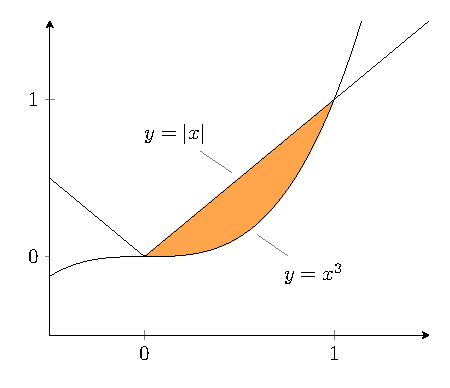
\includegraphics{../figures/quiz-3-1}
\caption{The area enclosed by the curves $y=|x|$ and $y=x^3$ at their
 points of intersection.}
 \label{fig:area-1}
\end{figure}
\\\\
(\ref{prob:2-ii}) As before, it helps to graph these curves (see Figure
\ref{fig:area-2}). From the figure we see that $y=e^{2x}$ and $e^{x}$
intersect at $x=0$ where $e^{2\cdot 0}=1=e^0$ and they both intersect the
vertical line $x=\ln 2$ at, well, obviously at $x=\ln 2$. So our integral
will be
\[
\int_0^{\ln 2}\left|e^{2x}-e^x\right|\diff x.
\]
Like before, note that $e^{2x}>e^x$ for any $0\leq x\leq \ln 2$ so we can
forget about the absolute value and evaluate the integral
\begin{align*}
\int_0^{\ln 2}e^{2x}-e^x\diff x
&=\left.\frac{e^{2x}}{2}-e^x\right|_0^{\ln 2}\\
&=\frac{e^{2\ln 2}}{2}-e^{\ln 2}-\left(\frac{e^{2\cdot 0}}{2}-e^{0} \right)\\
&=\frac{e^{\ln 2^2}}{2}-2-\left(\frac{1}{2}-1\right)\\
&=\frac{2^2}{2}-2+\frac{1}{2}\\
&=2-2+\frac{1}{2}\\
&=\boxed{\frac{1}{2}.}
\end{align*}
\begin{figure}[h]
\centering
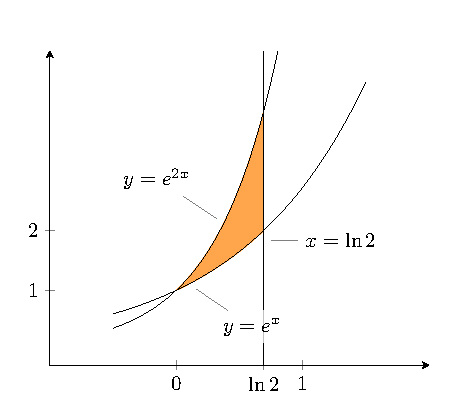
\includegraphics{../figures/quiz-3-2}
\caption{The area enclosed by the curves $y=e^x$, $y=e^{2x}$, and $x=\ln 2$
  at their points of intersection.}
 \label{fig:area-2}
\end{figure}
\end{proof}
\end{document}

%%% Local Variables:
%%% mode: latex
%%% TeX-master: t
%%% End:
